
\documentclass{standalone}
% font set
\usepackage{ctex}
\usepackage{fontspec}
\usepackage[T1]{fontenc}
\usepackage[sc]{mathpazo}
\usepackage{anyfontsize}
\setmainfont{Source Serif 4}
\setsansfont{Source Sans 3}
\setmonofont{Menlo}
\setCJKmainfont[BoldFont=黑体-简 中等,ItalicFont=楷体-简 常规体]{宋体-简 常规体}

% colors
\usepackage[dvipsnames]{xcolor}
\definecolor{pku-red}{RGB}{139,0,18}
\usepackage{colortbl}
\newcommand{\light}[1]{\textcolor{Orchid}{#1}}
\newcommand{\contrastlight}[1]{\textcolor{TealBlue}{#1}}

% plots
\usepackage{tikz}
\usepackage{tikz-cd}
\usetikzlibrary{arrows}
\usetikzlibrary{arrows.meta,positioning,calc,3d}
\usepackage{tikz-3dplot}
\usepackage{pgfplots}
\pgfplotsset{compat=newest}
\tikzset{
    punkt/.style={
        rectangle,
        rounded corners,
        draw=black, very thick,
        minimum height=2em,
        inner sep=6pt,
        text centered,
        fill=gray!30
    }
}

% math package
\let\Bbbk\relax
\usepackage{amsmath}
\usepackage{mathrsfs}
\usepackage{amssymb}
\usepackage{amsfonts}
\usepackage{stmaryrd}
\usepackage{latexsym}
\usepackage{extarrows}
\SetSymbolFont{stmry}{bold}{U}{stmry}{m}{n}


% math notations
\newcommand{\LHS}{\mathrm{LHS}}
\newcommand{\RHS}{\mathrm{RHS}}
\newcommand{\Z}{\mathbb{Z}}
\newcommand{\N}{\mathbb{N}}
\newcommand{\R}{\mathbb{R}}
\newcommand{\Q}{\mathbb{Q}}
\newcommand{\C}{\mathbb{C}}
\newcommand{\E}{\mathbb{E}}
\renewcommand{\O}{\mathcal{O}}
\newcommand{\id}{\mathrm{id}}
\DeclareMathOperator*{\Span}{Span}
\DeclareMathOperator*{\im}{Im}
\DeclareMathOperator*{\rank}{rank}
\DeclareMathOperator*{\card}{card}
\DeclareMathOperator*{\grad}{grad}
\DeclareMathOperator*{\argmax}{argmax}
\DeclareMathOperator*{\epi}{epi}
\DeclareMathOperator*{\maximize}{maximize}
\DeclareMathOperator*{\minimize}{minimize}
\renewcommand{\d}{\mathrm{d}}
\newcommand{\Pow}{\mathcal{P}}
\newcommand{\cov}{\mathsf{Cov}}
\newcommand{\var}{\mathsf{Var}}
\newcommand{\Nor}{\mathcal{N}}
\newcommand{\U}{\mathcal{U}}
\renewcommand{\t}{\mathsf{T}}
\newcommand{\T}{\top}
\newcommand{\F}{\bot}
\newcommand{\norm}[1]{\left\|#1\right\|}
\newcommand{\inner}[2]{\left\langle{#1},{#2}\right\rangle}
\newcommand{\e}{\mathrm{e}}
\newcommand{\const}{\mathrm{const}}
\newcommand{\scB}{\mathscr{B}}
\newcommand{\scF}{\mathscr{F}}
\newcommand{\G}{\mathscr{G}}
\newcommand{\Exp}{\mathsf{Exp}}
\newcommand{\DExp}{\mathsf{DExp}}
\newcommand{\Lap}{\mathsf{Lap}}
\newcommand{\calP}{\mathcal P}
\newcommand{\calS}{\mathcal S}
\newcommand{\calF}{\mathcal F}
\newcommand{\calM}{\mathcal M}
\newcommand{\KL}{\mathrm{KL}}
\newcommand{\ReLU}{\mathsf{ReLU}}
\newcommand{\val}{\mathsf{val}}

\DeclareSymbolFont{symbolsC}{U}{txsyc}{m}{n}
\DeclareMathSymbol{\strictif}{\mathrel}{symbolsC}{74}

\begin{document}
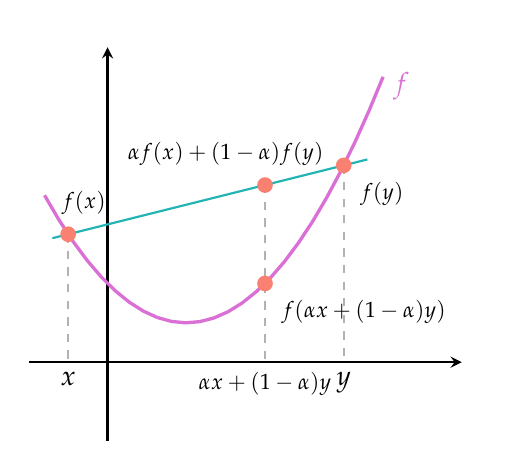
\begin{tikzpicture}[thick]
    \draw[-stealth] (-1,0) -- (4.5,0) node[right] {};
    \draw[-stealth] (0,-1) -- (0,4) node[above] {};
    \draw[TealBlue] (-0.5-0.2,1.625-0.2*0.875/3.5) -- (3+0.3,2.5+0.3*0.875/3.5);
    \draw[domain=-0.8:3.5,very thick,Orchid] plot (\x,{0.5*\x*\x-\x+1});
    \draw (3.5,3.5) node[right, Orchid] {$f$};
    \draw[dashed,gray!60] 
    (2,2.5-0.875/3.5) node[fill=Salmon,circle, draw=none, inner sep=2pt, label={[xshift=-0.5cm]above:{\footnotesize \textcolor{black}{$\alpha f(x) + (1-\alpha)f(y)$}}}] {} 
    -- 
    (2,1) node[fill=Salmon,circle, draw=none, inner sep=2pt, label={below right:{\footnotesize\textcolor{black}{$f(\alpha x + (1-\alpha)y)$}}}] {} 
    -- 
    (2,0) node[below,black,font=\footnotesize] {$\alpha x+(1-\alpha) y$};    

    \draw[dashed, gray!60] 
    (-0.5,1.625) node[fill=Salmon,circle, draw=none, inner sep=2pt,label={[xshift=0.2cm]above:{\footnotesize \textcolor{black}{$f(x)$}}}] {} 
    -- 
    (-0.5,0) node[below,black] {$x$};
    \draw[dashed, gray!60] (3,2.5) node[fill=Salmon,circle, draw=none, inner sep=2pt,label={below right:{\footnotesize \textcolor{black}{$f(y)$}}}] {} 
    --
    (3,0) node[below,black] {$y$};
\end{tikzpicture}
\end{document}